
%(BEGIN_QUESTION)
% Copyright 2011, Tony R. Kuphaldt, released under the Creative Commons Attribution License (v 1.0)
% This means you may do almost anything with this work of mine, so long as you give me proper credit

Anta at en instrumenttekniker kobler et oscilloskop til et FOUNDATION Fieldbus-segment som vist, med hensikt å se signalet:

$$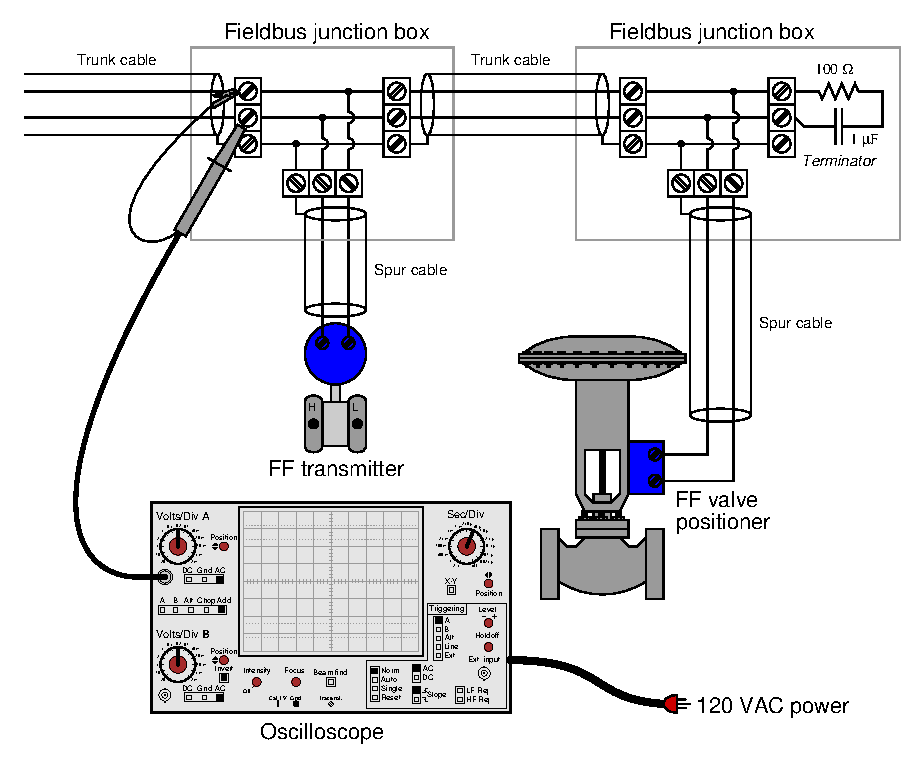
\includegraphics[width=15.5cm]{i00890x01.eps}$$

Forklar hva som er galt med oppsettet, og hvilke problemer det kan gi i segmentet. Hvordan {\it bør} oscilloskopet kobles til segmentkabelen?

\vskip 20pt \vbox{\hrule \hbox{\strut \vrule{} {\bf Forslag til sokratisk diskusjon} \vrule} \hrule}

\begin{itemize}
\item{} Forklar hvordan slik feil bruk av oscilloskop kan utgjøre en {\it sikkerhetsrisiko} for teknikeren i andre kretstyper (ikke bare Fieldbus H1).
\item{} En vanlig praksis for å omgå problemet er å forsyne oscilloskopet via {\it isolasjonstransformator} slik at AC-forsyningen blir ujordet. Forklar hvordan dette løser måleproblemet i diagrammet, og hvorfor praksisen likevel kan være utrygg.
\end{itemize}

\underbar{file i00890}
%(END_QUESTION)





%(BEGIN_ANSWER)

Å koble et nettforsynt oscilloskop til FF-segmentet på denne måten skaper en {\it jordfeil} i systemet, som i verste fall kan slå ut kommunikasjonen i hele segmentet.

%(END_ANSWER)





%(BEGIN_NOTES)

Oscilloskopet bør settes opp for {\it differensiell} måling, der to inngangskanaler brukes, og ingen jordklemmer kobles til noen punkt i FF-segmentet.

%INDEX% Electronics review: oscilloscope usage
%INDEX% Fieldbus, FOUNDATION (H1): segment troubleshooting

%(END_NOTES)
